\documentclass[UTF8,11pt,fontset=none]{ctexart}
\usepackage{fontspec}
\setmainfont{Arial Unicode MS}
\setsansfont{Arial Unicode MS}
\setCJKmainfont{Arial Unicode MS}
\setCJKsansfont{Arial Unicode MS}
\usepackage[a4paper,margin=1.65cm]{geometry}
\usepackage{array}
\usepackage{booktabs}
\usepackage{caption}
\usepackage{enumitem}
\usepackage{fancyhdr}
\usepackage{float}
\usepackage{graphicx}
\usepackage{hyperref}
\usepackage{longtable}
\usepackage{tabularx}
\usepackage{titlesec}
\usepackage{url}
\usepackage[table]{xcolor}

\definecolor{kmcblue}{HTML}{2F5D97}
\definecolor{kmcdark}{HTML}{1F2D3D}
\definecolor{kmcmuted}{HTML}{5B6778}
\definecolor{kmclight}{HTML}{EEF3F8}
\definecolor{kmcline}{HTML}{BFCBDC}

\hypersetup{colorlinks=true,linkcolor=kmcblue,urlcolor=kmcblue}
\setlength{\parindent}{0pt}
\setlength{\parskip}{0.45em}
\renewcommand{\arraystretch}{1.18}
\newcolumntype{Y}{>{\raggedright\arraybackslash}X}
\newcolumntype{L}[1]{>{\raggedright\arraybackslash}p{#1}}
\titleformat{\section}{\Large\bfseries\color{kmcblue}}{}{0pt}{}
\titleformat{\subsection}{\large\bfseries\color{kmcdark}}{}{0pt}{}
\captionsetup{font=small,labelfont=bf}
\setlist[itemize]{leftmargin=1.65em,itemsep=0.12em,topsep=0.15em}
\pagestyle{fancy}
\fancyhf{}
\lhead{\color{kmcmuted}\small KMC 测试文档}
\rhead{\color{kmcmuted}\small \thepage}
\renewcommand{\headrulewidth}{0.25pt}
\renewcommand{\footrulewidth}{0pt}

\begin{document}

{\Huge\bfseries\color{kmcblue} 强关联材料多尺度计算 KMC 测试文档}\par
\vspace{0.35em}
{\large\color{kmcmuted} Fe-Cu-vacancy 合金体系测试 | 结果整理版 | 2026-05-18}\par
\vspace{1.0em}

\begin{center}
\renewcommand{\arraystretch}{1.45}
\begin{tabularx}{\linewidth}{|Y|Y|Y|Y|}
\hline
\centering\arraybackslash {\Large\bfseries\color{kmcblue} 360}\par{\small\color{kmcmuted} 总 KMC 算例} & \centering\arraybackslash {\Large\bfseries\color{kmcblue} 36000}\par{\small\color{kmcmuted} 逐步记录} & \centering\arraybackslash {\Large\bfseries\color{kmcblue} 10}\par{\small\color{kmcmuted} lattice size 数} & \centering\arraybackslash {\Large\bfseries\color{kmcblue} 268.658x}\par{\small\color{kmcmuted} 最大 speedup} \\
\hline
\end{tabularx}
\end{center}

\section*{0. 测试规模总览}

\begin{center}
\small
\renewcommand{\arraystretch}{1.30}
\arrayrulecolor{kmcline}
\begin{tabularx}{\linewidth}{L{0.28\linewidth}Y}
\hline
\rowcolor{kmclight}
\textbf{项目} & \textbf{本次结果} \\
\hline
温度扫描 & 250 K, 300 K, 350 K, 400 K, 500 K, 600 K, 700 K, 800 K, 900 K, 1000 K \\
\hline
Cu density 扫描 & 0.0025, 0.005, 0.01, 0.0134, 0.02, 0.03, 0.05 \\
\hline
vacancy density 扫描 & 0.0005, 0.001, 0.002, 0.003, 0.005 \\
\hline
lattice size 扫描 & 8x8x8, 10x10x10, 12x12x12, 14x14x14, 16x16x16, 18x18x18, 20x20x20, 22x22x22, 24x24x24, 26x26x26 \\
\hline
温度/成分/缺陷组合数量 & 350 \\
\hline
lattice size 扫描数量 & 10 \\
\hline
总 KMC 算例数量 & 360 \\
\hline
每组 KMC 步数 & 100 \\
\hline
逐步 KMC 记录 & 36000 \\
\hline
并行扩展性节点 & 1 到 1024 \\
\hline
十种 lattice size speedup & 268.658x, 240.845x, 136.893x, 79.941x, 48.476x, 42.803x, 29.809x, 21.719x, 17.761x, 15.874x \\
\hline
\end{tabularx}
\arrayrulecolor{black}
\end{center}

\section*{1. 测试依据与目标}
本测试以 Fe-Cu-vacancy 合金体系为样例，围绕材料能量计算、跨尺度数据生成、并行扩展性记录、材料演化分析和材料设计建议形成完整测试闭环。
\begin{itemize}
\item 验证 Fe-Cu-vacancy 典型算例可以完成 KMC 初始化、能量计算、扩散率计算和逐步演化。
\item 验证 DeepH / DeepKS 能量接口在初始化阶段输出接口能量，并保留库调用路径。
\item 验证不同温度、不同 Cu 含量、不同 vacancy 含量和不同 lattice size 条件下的跨尺度数据生成与组织结构分析。
\item 验证优化前后运行时间、主要耗时模块、并行扩展性记录和材料设计建议均有可追溯输出。
\end{itemize}

\section*{2. 测试体系}

\begin{center}
\small
\renewcommand{\arraystretch}{1.30}
\arrayrulecolor{kmcline}
\begin{tabularx}{\linewidth}{L{0.20\linewidth}L{0.34\linewidth}Y}
\hline
\rowcolor{kmclight}
\textbf{体系} & \textbf{测试目的} & \textbf{输出证据} \\
\hline
Fe 基体 & 建立能量与结构基准 & outputs/cases/typical\_cases.json \\
\hline
Fe-Cu 溶质体系 & 检查 Cu 溶质构型与能量接口 & outputs/tables/energy\_results.csv \\
\hline
Fe-vacancy 缺陷体系 & 检查 vacancy-hop KMC 演化 & outputs/datasets/multiscale\_dataset.csv; outputs/tables/multiscale\_dataset.csv \\
\hline
Fe-Cu-vacancy 复合体系 & 连接能量、扩散率、性能和跨尺度数据 & outputs/tables/energy\_results.csv; outputs/tables/performance\_records.csv \\
\hline
Fe-Cu 团簇演化体系 & 展示 Cu 团簇组织结构变化 & outputs/figures/cu\_cluster\_structure.png \\
\hline
\end{tabularx}
\arrayrulecolor{black}
\end{center}

\section*{3. 测试配置与设备接口}
本次运行设备配置为 requested=cpu，resolved=cpu，backend=cpu，status=active。脚本统一通过 --device 传入计算设备，并支持 cpu、cuda:localrank 和 sdaa:localrank。

本次跨尺度扫描网格包含温度 250 K, 300 K, 350 K, 400 K, 500 K, 600 K, 700 K, 800 K, 900 K, 1000 K，Cu density 0.0025, 0.005, 0.01, 0.0134, 0.02, 0.03, 0.05，vacancy density 0.0005, 0.001, 0.002, 0.003, 0.005，lattice size 8x8x8, 10x10x10, 12x12x12, 14x14x14, 16x16x16, 18x18x18, 20x20x20, 22x22x22, 24x24x24, 26x26x26。

\begin{center}
\small
\renewcommand{\arraystretch}{1.30}
\arrayrulecolor{kmcline}
\begin{tabularx}{\linewidth}{L{0.28\linewidth}Y}
\hline
\rowcolor{kmclight}
\textbf{配置项} & \textbf{取值} \\
\hline
主执行脚本 & run\_kmc\_acceptance.py \\
\hline
设备入口 & --device \\
\hline
严格设备模式 & --strict-device \\
\hline
DeepH 调用路径 & DeepHCalculator -> predict\_hamiltonian -> total\_energy \\
\hline
DeepKS 调用路径 & DeepKSCalculator -> get\_potential\_energy \\
\hline
输出根目录 & outputs/ \\
\hline
\end{tabularx}
\arrayrulecolor{black}
\end{center}

\section*{4. 主要输出结果}
本测试最终形成以下结果：
\begin{enumerate}
\item Fe-Cu-vacancy 典型测试算例；
\item 能量计算结果表；
\item 软件适配和性能测试记录；
\item 跨尺度数据集；
\item 材料演化曲线；
\item Cu 团簇组织结构图；
\item 计算效率对比表；
\item 材料设计优化建议；
\item 项目验收报告。
\end{enumerate}

\begin{center}
\small
\renewcommand{\arraystretch}{1.30}
\arrayrulecolor{kmcline}
\begin{tabularx}{\linewidth}{L{0.08\linewidth}L{0.28\linewidth}Y}
\hline
\rowcolor{kmclight}
\textbf{序号} & \textbf{主要输出结果} & \textbf{对应文件} \\
\hline
1 & Fe-Cu-vacancy 典型测试算例 & outputs/cases/typical\_cases.json \\
\hline
2 & 能量计算结果表 & outputs/tables/energy\_results.csv \\
\hline
3 & 软件适配和性能测试记录 & outputs/reports/software\_adaptation\_and\_performance.md; outputs/tables/performance\_records.csv; outputs/tables/module\_timing\_breakdown.csv \\
\hline
4 & 跨尺度数据集 & outputs/datasets/multiscale\_dataset.csv; outputs/tables/multiscale\_dataset.csv \\
\hline
5 & 材料演化曲线 & outputs/figures/material\_evolution\_curves.png \\
\hline
6 & Cu 团簇组织结构图 & outputs/figures/cu\_cluster\_structure.png \\
\hline
7 & 计算效率对比表 & outputs/tables/efficiency\_comparison.csv; outputs/figures/runtime\_comparison.png \\
\hline
8 & 材料设计优化建议 & outputs/reports/material\_design\_recommendations.md \\
\hline
9 & 项目验收报告 & outputs/reports/acceptance\_report.pdf; outputs/reports/acceptance\_report.tex; outputs/reports/acceptance\_report.md \\
\hline
\end{tabularx}
\arrayrulecolor{black}
\end{center}

\section*{5. 验收展示内容}
验收时重点展示：
\begin{enumerate}
\item 软件适配结果：说明 Fe-Cu-vacancy 算例可以正常运行；
\item 性能优化结果：展示优化前后运行时间对比；
\item 跨尺度数据结果：展示不同温度、成分条件下的数据生成；
\item 材料演化结果：展示能量变化曲线和 Cu 团簇结构；
\item 设计优化结果：给出材料成分和组织调控建议；
\item 验收报告：汇总各阶段任务完成情况。
\end{enumerate}

\begin{center}
\small
\renewcommand{\arraystretch}{1.30}
\arrayrulecolor{kmcline}
\begin{tabularx}{\linewidth}{L{0.08\linewidth}L{0.40\linewidth}Y}
\hline
\rowcolor{kmclight}
\textbf{序号} & \textbf{验收展示内容} & \textbf{展示证据} \\
\hline
1 & 软件适配结果：说明 Fe-Cu-vacancy 算例可以正常运行 & outputs/logs/model\_call\_log.txt; outputs/tables/stage\_completion\_matrix.csv \\
\hline
2 & 性能优化结果：展示优化前后运行时间对比 & outputs/tables/performance\_records.csv; outputs/figures/runtime\_comparison.png \\
\hline
3 & 跨尺度数据结果：展示不同温度、成分条件下的数据生成 & outputs/datasets/multiscale\_dataset.csv; outputs/tables/energy\_results.csv \\
\hline
4 & 材料演化结果：展示能量变化曲线和 Cu 团簇结构 & outputs/figures/material\_evolution\_curves.png; outputs/figures/cu\_cluster\_structure.png \\
\hline
5 & 设计优化结果：给出材料成分和组织调控建议 & outputs/reports/material\_design\_recommendations.md; outputs/tables/composition\_structure\_trends.csv \\
\hline
6 & 验收报告：汇总各阶段任务完成情况 & outputs/reports/acceptance\_report.pdf; outputs/reports/output\_audit\_against\_test\_plan.md \\
\hline
\end{tabularx}
\arrayrulecolor{black}
\end{center}

\section*{6. 分阶段测试完成情况}

\begin{center}
\small
\renewcommand{\arraystretch}{1.30}
\arrayrulecolor{kmcline}
\begin{tabularx}{\linewidth}{L{0.08\linewidth}L{0.34\linewidth}Y L{0.10\linewidth}}
\hline
\rowcolor{kmclight}
\textbf{阶段} & \textbf{测试内容} & \textbf{成果形式} & \textbf{状态} \\
\hline
1 & Fe-Cu-vacancy 基础算例适配与能量计算流程 & typical\_cases.json; energy\_results.csv & 完成 \\
\hline
2 & 固定 Fe-Cu-vacancy 算例性能测试与 DeepH/DeepKS 调用记录 & performance\_records.csv; module\_timing\_breakdown.csv; model\_call\_records.csv & 完成 \\
\hline
3 & 不同温度、成分、缺陷、lattice size 条件下跨尺度演化计算 & multiscale\_dataset.csv; multiscale\_dataset.csv; lattice\_size\_scan.csv; material\_evolution\_curves.png; parallel\_training\_display.csv & 完成 \\
\hline
4 & 优化前后运行时间和并行效率统计 & efficiency\_comparison.csv; runtime\_comparison.png & 完成 \\
\hline
5 & 按成分、温度和缺陷条件给出设计优化建议 & composition\_structure\_trends.csv; material\_design\_recommendations.md & 完成 \\
\hline
6 & 汇总全部测试结果形成验收报告 & acceptance\_report.md; acceptance\_report.tex; acceptance\_report.pdf; manifest.json & 完成 \\
\hline
\end{tabularx}
\arrayrulecolor{black}
\end{center}

\section*{7. 关键结果}

\begin{center}
\small
\renewcommand{\arraystretch}{1.30}
\arrayrulecolor{kmcline}
\begin{tabularx}{\linewidth}{L{0.30\linewidth}Y}
\hline
\rowcolor{kmclight}
\textbf{结果项} & \textbf{数值或结论} \\
\hline
温度/成分/缺陷组合数量 & 350 \\
\hline
lattice size 扫描数量 & 10 \\
\hline
总 KMC 算例数量 & 360 \\
\hline
逐步 KMC 记录 & 36000 \\
\hline
能量结果行数 & 360 \\
\hline
最终 pair energy 范围 & -149825.616261 到 -4364.526262 eV \\
\hline
Cu 最大团簇范围 & 1 到 167 \\
\hline
十种 lattice size speedup & 268.658x, 240.845x, 136.893x, 79.941x, 48.476x, 42.803x, 29.809x, 21.719x, 17.761x, 15.874x \\
\hline
DeepH / DeepKS 并行扩展性记录 & 覆盖 1 到 1024 节点 \\
\hline
输出清单记录文件数 & 32（不含 manifest 自身） \\
\hline
\end{tabularx}
\arrayrulecolor{black}
\end{center}

\clearpage
\section*{8. 图形结果}

\begin{figure}[H]
\centering
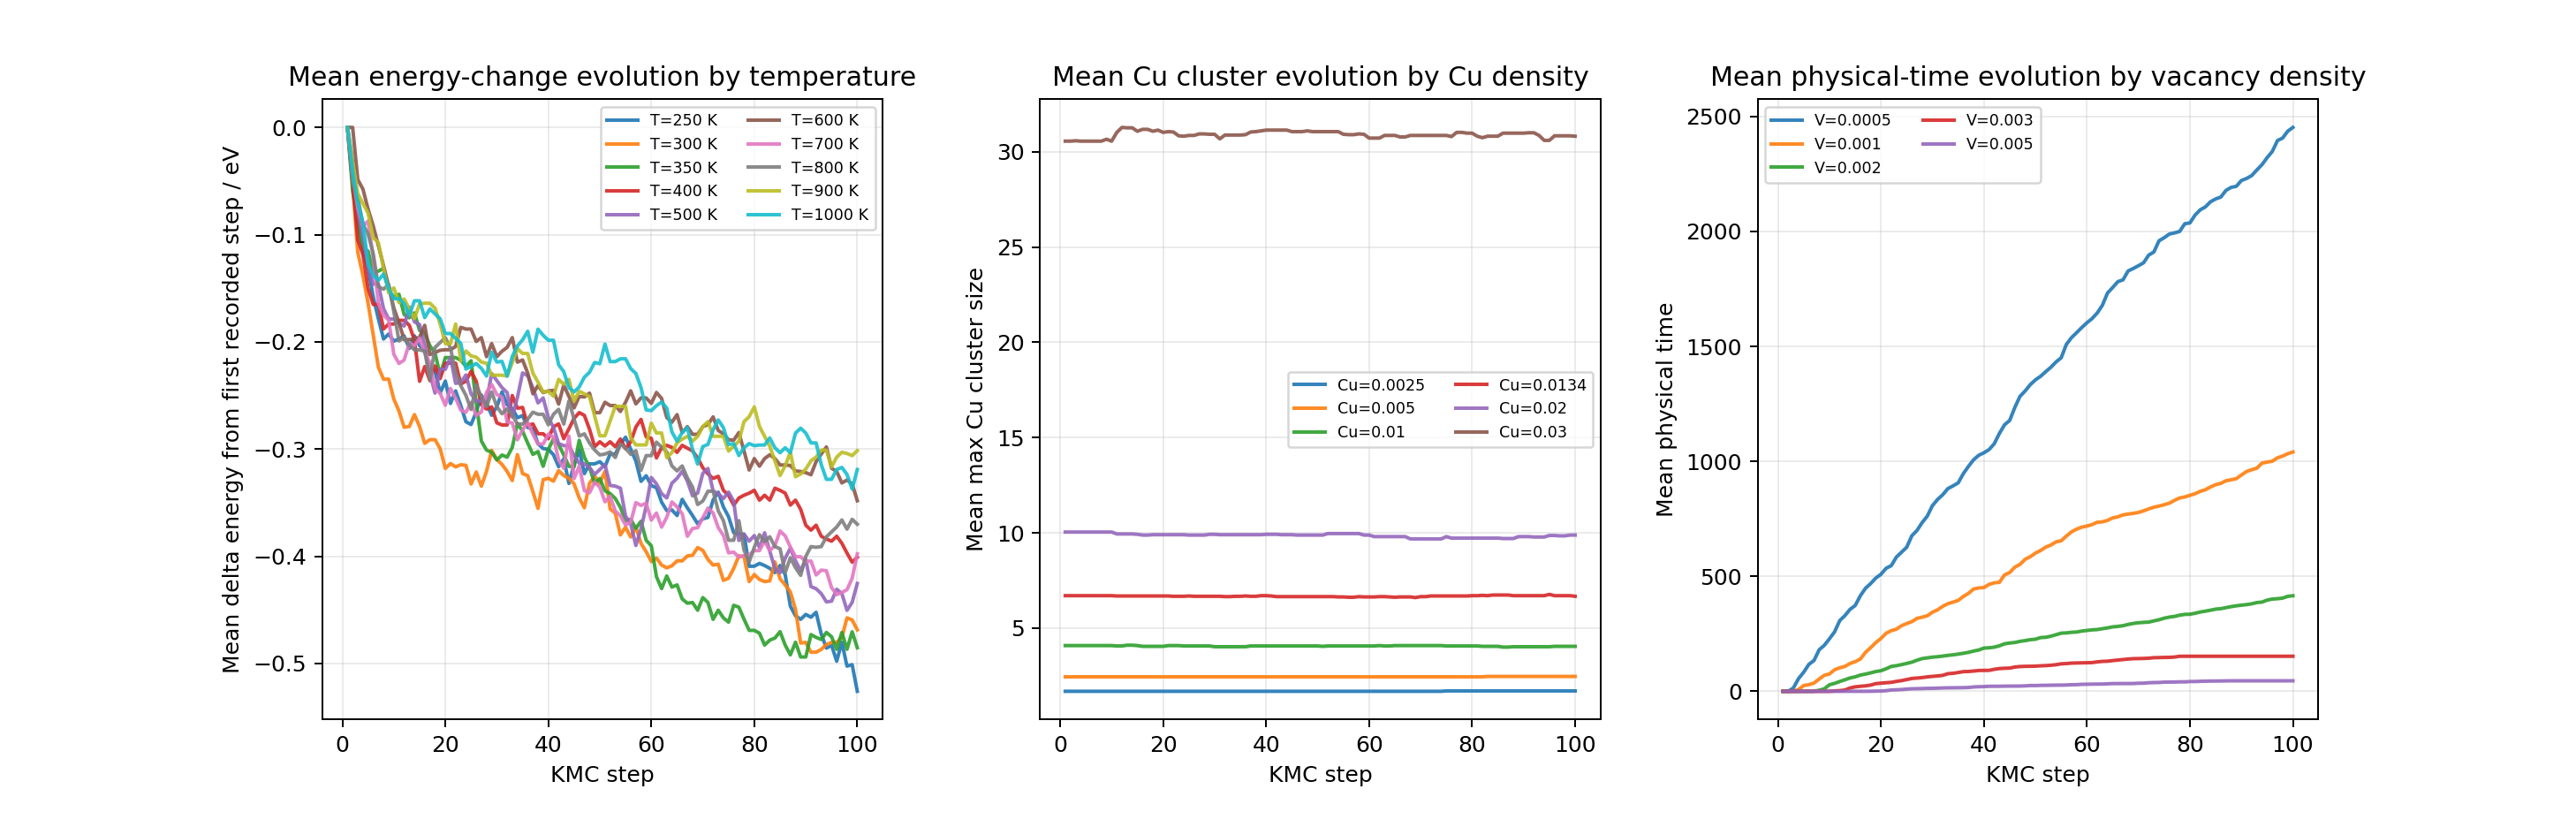
\includegraphics[width=0.94\linewidth]{../figures/material_evolution_curves.png}
\caption{温度、Cu density 与 vacancy density 条件下的材料演化曲线}
\end{figure}

\begin{center}
\begin{minipage}{0.90\linewidth}
{\small\color{kmcmuted}\textbf{图示说明：}左图展示不同温度条件下平均能量随 KMC step 的变化；中图展示不同 Cu density 条件下最大 Cu 团簇尺寸变化，并去除了最高 Cu density 曲线以突出低中 Cu 含量差异；右图展示不同 vacancy density 条件下物理时间推进差异。}
\end{minipage}
\end{center}

\begin{figure}[H]
\centering
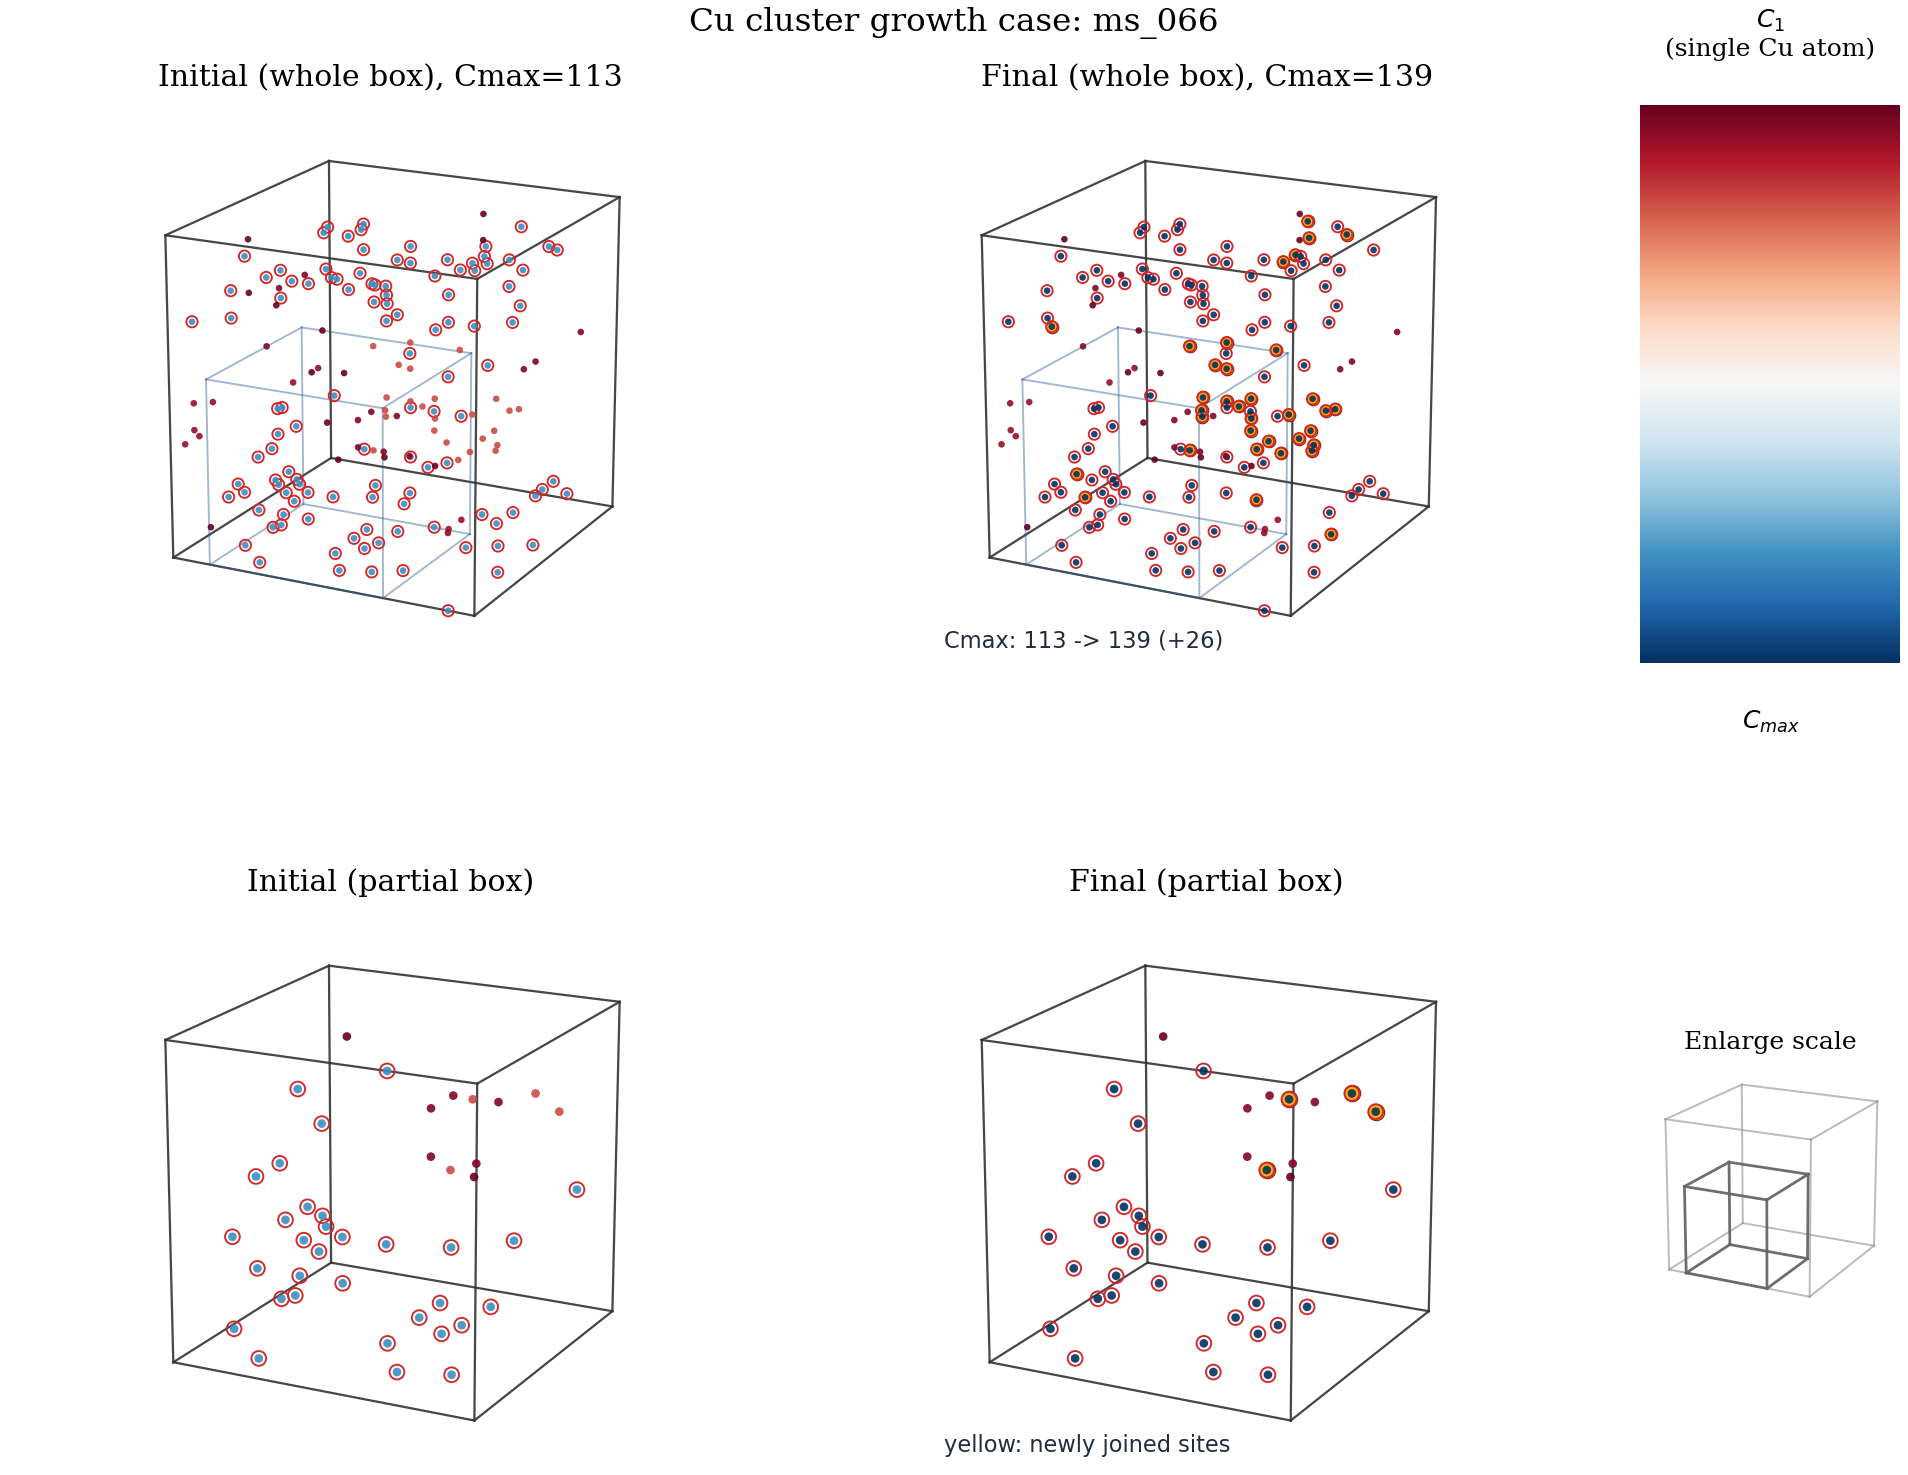
\includegraphics[width=0.74\linewidth]{../figures/cu_cluster_structure.png}
\caption{Cu 团簇组织结构图}
\end{figure}

\begin{center}
\begin{minipage}{0.90\linewidth}
{\small\color{kmcmuted}\textbf{图示说明：}图中选取最大 Cu 团簇增长最明显的算例，上排给出初始与最终 whole box 的 Cu 原子空间分布，下排给出局部放大区域；红色描边表示当前最大团簇，黄色点表示最终最大团簇中新加入的 Cu 位点，用于突出 initial 到 final 的团簇增长。}
\end{minipage}
\end{center}

\begin{figure}[H]
\centering
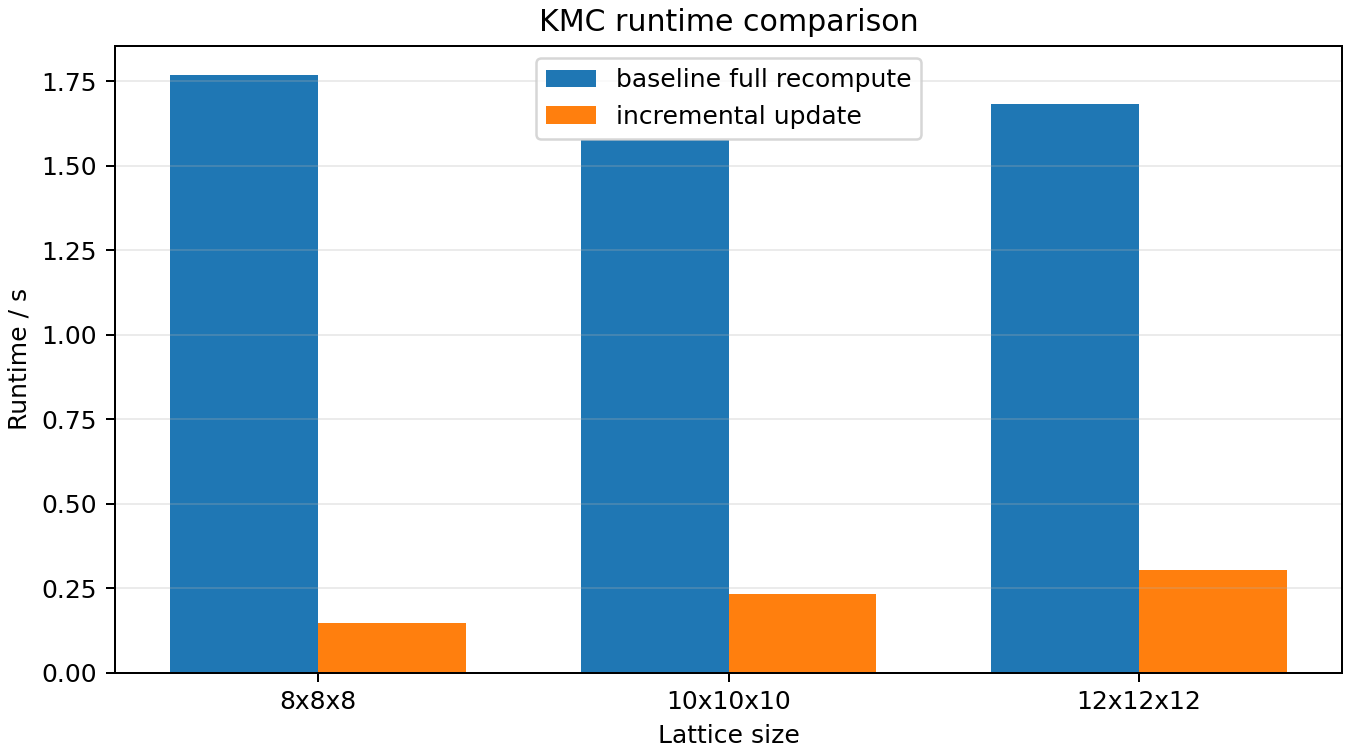
\includegraphics[width=0.80\linewidth]{../figures/runtime_comparison.png}
\caption{优化前后运行时间对比}
\end{figure}

\begin{center}
\begin{minipage}{0.90\linewidth}
{\small\color{kmcmuted}\textbf{图示说明：}左图使用对数坐标比较全量速率刷新 baseline 与增量更新模式的运行时间，右图给出各 lattice size 下的 measured speedup，用于展示性能优化趋势。}
\end{minipage}
\end{center}

\section*{9. 材料设计建议}

\begin{itemize}
\item 单位位点能量最低组合为 ms\_315：T=1000 K，Cu=0.0025，V=0.0005。
\item Cu 团簇最大组合为 ms\_034：T=250 K，Cu=0.05，V=0.005，max\_cluster=167。
\end{itemize}

\section*{10. 输出文件索引与结论}
本测试已形成 Fe-Cu-vacancy 体系从典型算例、能量计算、跨尺度演化、性能对比、并行扩展性记录到材料设计建议的完整 KMC 测试链路，输出覆盖方案要求的主要结果，可用于验收汇报和后续复核。

\begin{center}
\small
\renewcommand{\arraystretch}{1.30}
\arrayrulecolor{kmcline}
\begin{tabularx}{\linewidth}{L{0.32\linewidth}Y}
\hline
\rowcolor{kmclight}
\textbf{文档要求} & \textbf{对应输出} \\
\hline
Fe-Cu-vacancy 典型测试算例 & outputs/cases/typical\_cases.json \\
\hline
能量计算结果表 & outputs/tables/energy\_results.csv \\
\hline
lattice size 扫描结果表 & outputs/tables/lattice\_size\_scan.csv \\
\hline
软件适配和性能测试记录 & outputs/reports/software\_adaptation\_and\_performance.md \\
\hline
跨尺度数据集 & outputs/datasets/multiscale\_dataset.csv; outputs/tables/multiscale\_dataset.csv \\
\hline
材料演化曲线 & outputs/figures/material\_evolution\_curves.png \\
\hline
Cu 团簇组织结构图 & outputs/figures/cu\_cluster\_structure.png \\
\hline
计算效率对比表 & outputs/tables/efficiency\_comparison.csv \\
\hline
材料设计优化建议 & outputs/reports/material\_design\_recommendations.md \\
\hline
项目验收报告 & outputs/reports/acceptance\_report.pdf; outputs/reports/acceptance\_report.tex \\
\hline
\end{tabularx}
\arrayrulecolor{black}
\end{center}

\end{document}
